% !TEX root = ../../main.tex

% Numerical experiments section
\subsection{Experiments}
\label{sec:experiments}

To demonstrate the %validity and
empirical performance of iPMCMC we report experiments on two state space models.  
Although both the models considered are Markovian, we emphasise that iPMCMC goes far beyond this and can be applied to arbitrary graphical models
and even probabilistic programs as explained in Section~\ref{sec:proginf:str:part:ipmcmc}. 
%For exposition we will focus our comparison to the trivial distribution, whereby $M$ independent PMCMC samplers are run in parallel, of PG, particle independent Metropolis-Hastings (PIMH) \cite{andrieuDH2010} and the alternate move PG sampler (APG) \cite{holenstein2009particle}. 
We will focus our comparison on the trivially distributed alternatives, whereby $M$ independent PMCMC samplers are run in parallel--these are PG, particle independent Metropolis-Hastings (PIMH) \citep{andrieuDH2010} and the alternate move PG sampler (APG) \citep{holenstein2009particle}. Comparisons to other alternatives, including independent SMC, serialized implementations of PG and PIMH, and running a mixture of independent PG and PIMH samplers, are provided in the supplementary material of~\cite{rainforth2016interacting}.  
None outperformed the methods considered here, with the exception of running a serialized PG implementation with an increased number of particles, requiring significant additional memory ($O(MN)$ as opposed to $O(M+N)$).

APG interleaves PG steps with PIMH steps
%, alternating between \csmc updates and a Metropolis-Hastings step with an independent \smc proposal,
in an attempt to overcome the issues caused by path degeneracy in PG.  We refer to the trivially distributed versions of these algorithms as multi-start PG, PIMH and APG respectively (mPG, mPIMH and mAPG). 
We use Rao-Blackwellization, as described in \ref{sec:part:ipmcmc:allparticles}, to average over all the generated particles for all methods, weighting the independent Markov chains equally for mPG, mPIMH and mAPG. We note that mPG is a special case of iPMCMC for which $P=M$.  Because our interest is in alleviating degeneracy, we used the bootstrap proposal and multinomial resampling in our experiments.\footnote{However, we recommend
	using systematic resampling, as is the default in the provided implementations.}
 $M=32$ nodes and $N=100$ particles were used unless otherwise stated.  Initialization of the retained particles for iPMCMC and mPG was done by using standard SMC sweeps.

\subsubsection{Linear Gaussian State Space Model}
\label{sec:LGSS}
We first consider a linear Gaussian state space model (LGSSM) with 3 dimensional latent states $x_{1:T}$, 20 dimensional observations $y_{1:T}$ and dynamics given by %\cn{It seems you use deterministic initial conditions for $x_0$, reformulate the model so you have a prior $\mu(x_1)$ instead? (also follows notation above)}
\begin{subequations}
	\label{eq:LGSS}
	\vspace{-6pt}
	\begin{align}
	\vspace{-6pt}
	x_1 & \sim \mathcal{N} \left(\mu, V\right) \label{eq:LGSSa} \displaybreak[0]\\
	\vspace{-6pt}
	x_t & = \alpha x_{t-1} + \delta_{t-1} \quad & \delta_{t-1} \sim \mathcal{N} \left(0, \Omega\right) \label{eq:LGSSb} \displaybreak[0] \\
	\vspace{-6pt}
	y_t & = \beta x_{t} + \varepsilon_{t} \quad & \varepsilon_{t} \sim \mathcal{N} \left(0, \Sigma\right).
	\label{eq:LGSSc}
	\end{align}
\end{subequations}
We set $\mu = [0, 1, 1]^T$, $V = 0.1 \; \mathbf{I}$, $\Omega = \mathbf{I}$ and $\Sigma = 0.1 \; \mathbf{I}$ where $\mathbf{I}$ represents the identity matrix.  The constant transition matrix, $\alpha$, corresponds to successively applying rotations of $\frac{7\pi}{10}$, $\frac{3\pi}{10}$ and $\frac{\pi}{20}$ about the first, second and third dimensions of $x_{t-1}$ respectively followed by a scaling of $0.99$ to ensure that the dynamics remain stable.  A total of 10 different synthetic datasets of length $T=50$ were generated by simulating from~\eqref{eq:LGSSa}--\eqref{eq:LGSSc}, each with a different emission matrix $\beta$ generated by sampling each column independently from a symmetric Dirichlet distribution with concentration parameter 0.2.

\begin{figure*}[t]
	\centering
	\begin{subfigure}[t]{0.49\textwidth}
		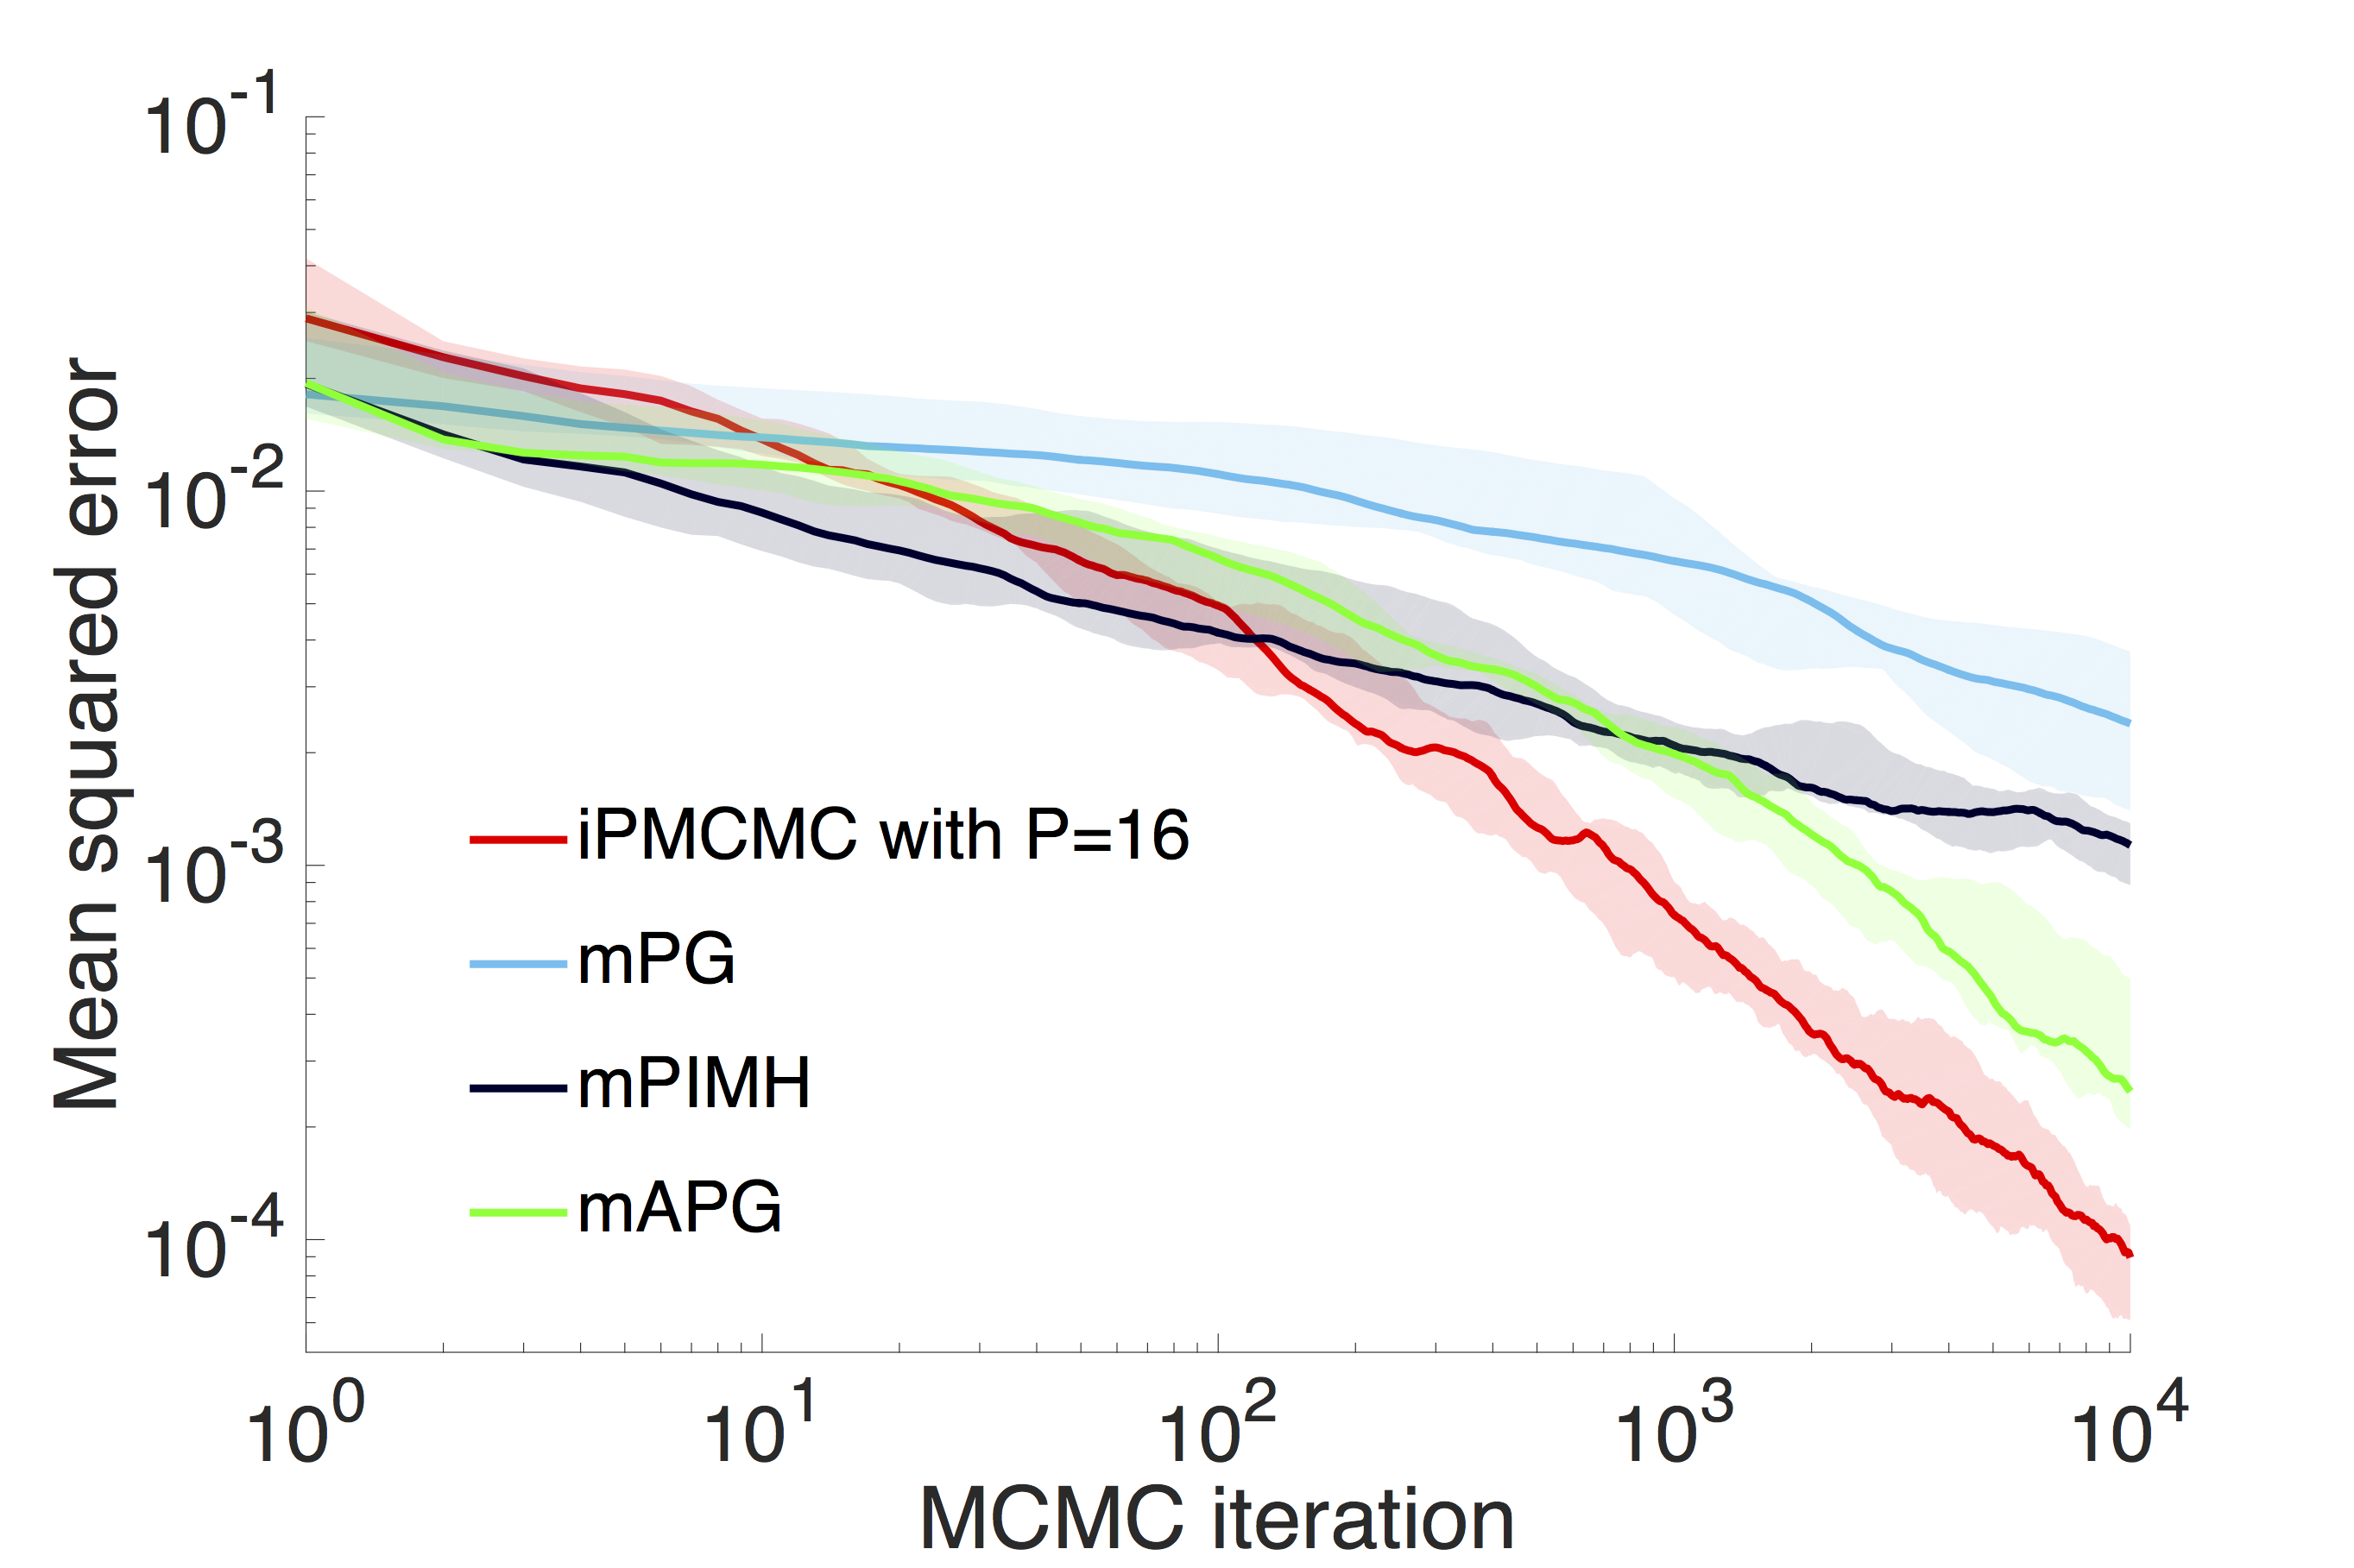
\includegraphics[width=0.98\textwidth]{mean_conv_lss}
		\caption{Convergence in mean for full sequence}
		\label{fig:meanConv}
	\end{subfigure}
	~  %add desired spacing between images, e. g. ~, \quad, \qquad, \hfill etc. 
	%(or a blank line to force the subfigure onto a new line)
	\begin{subfigure}[t]{0.49\textwidth}
		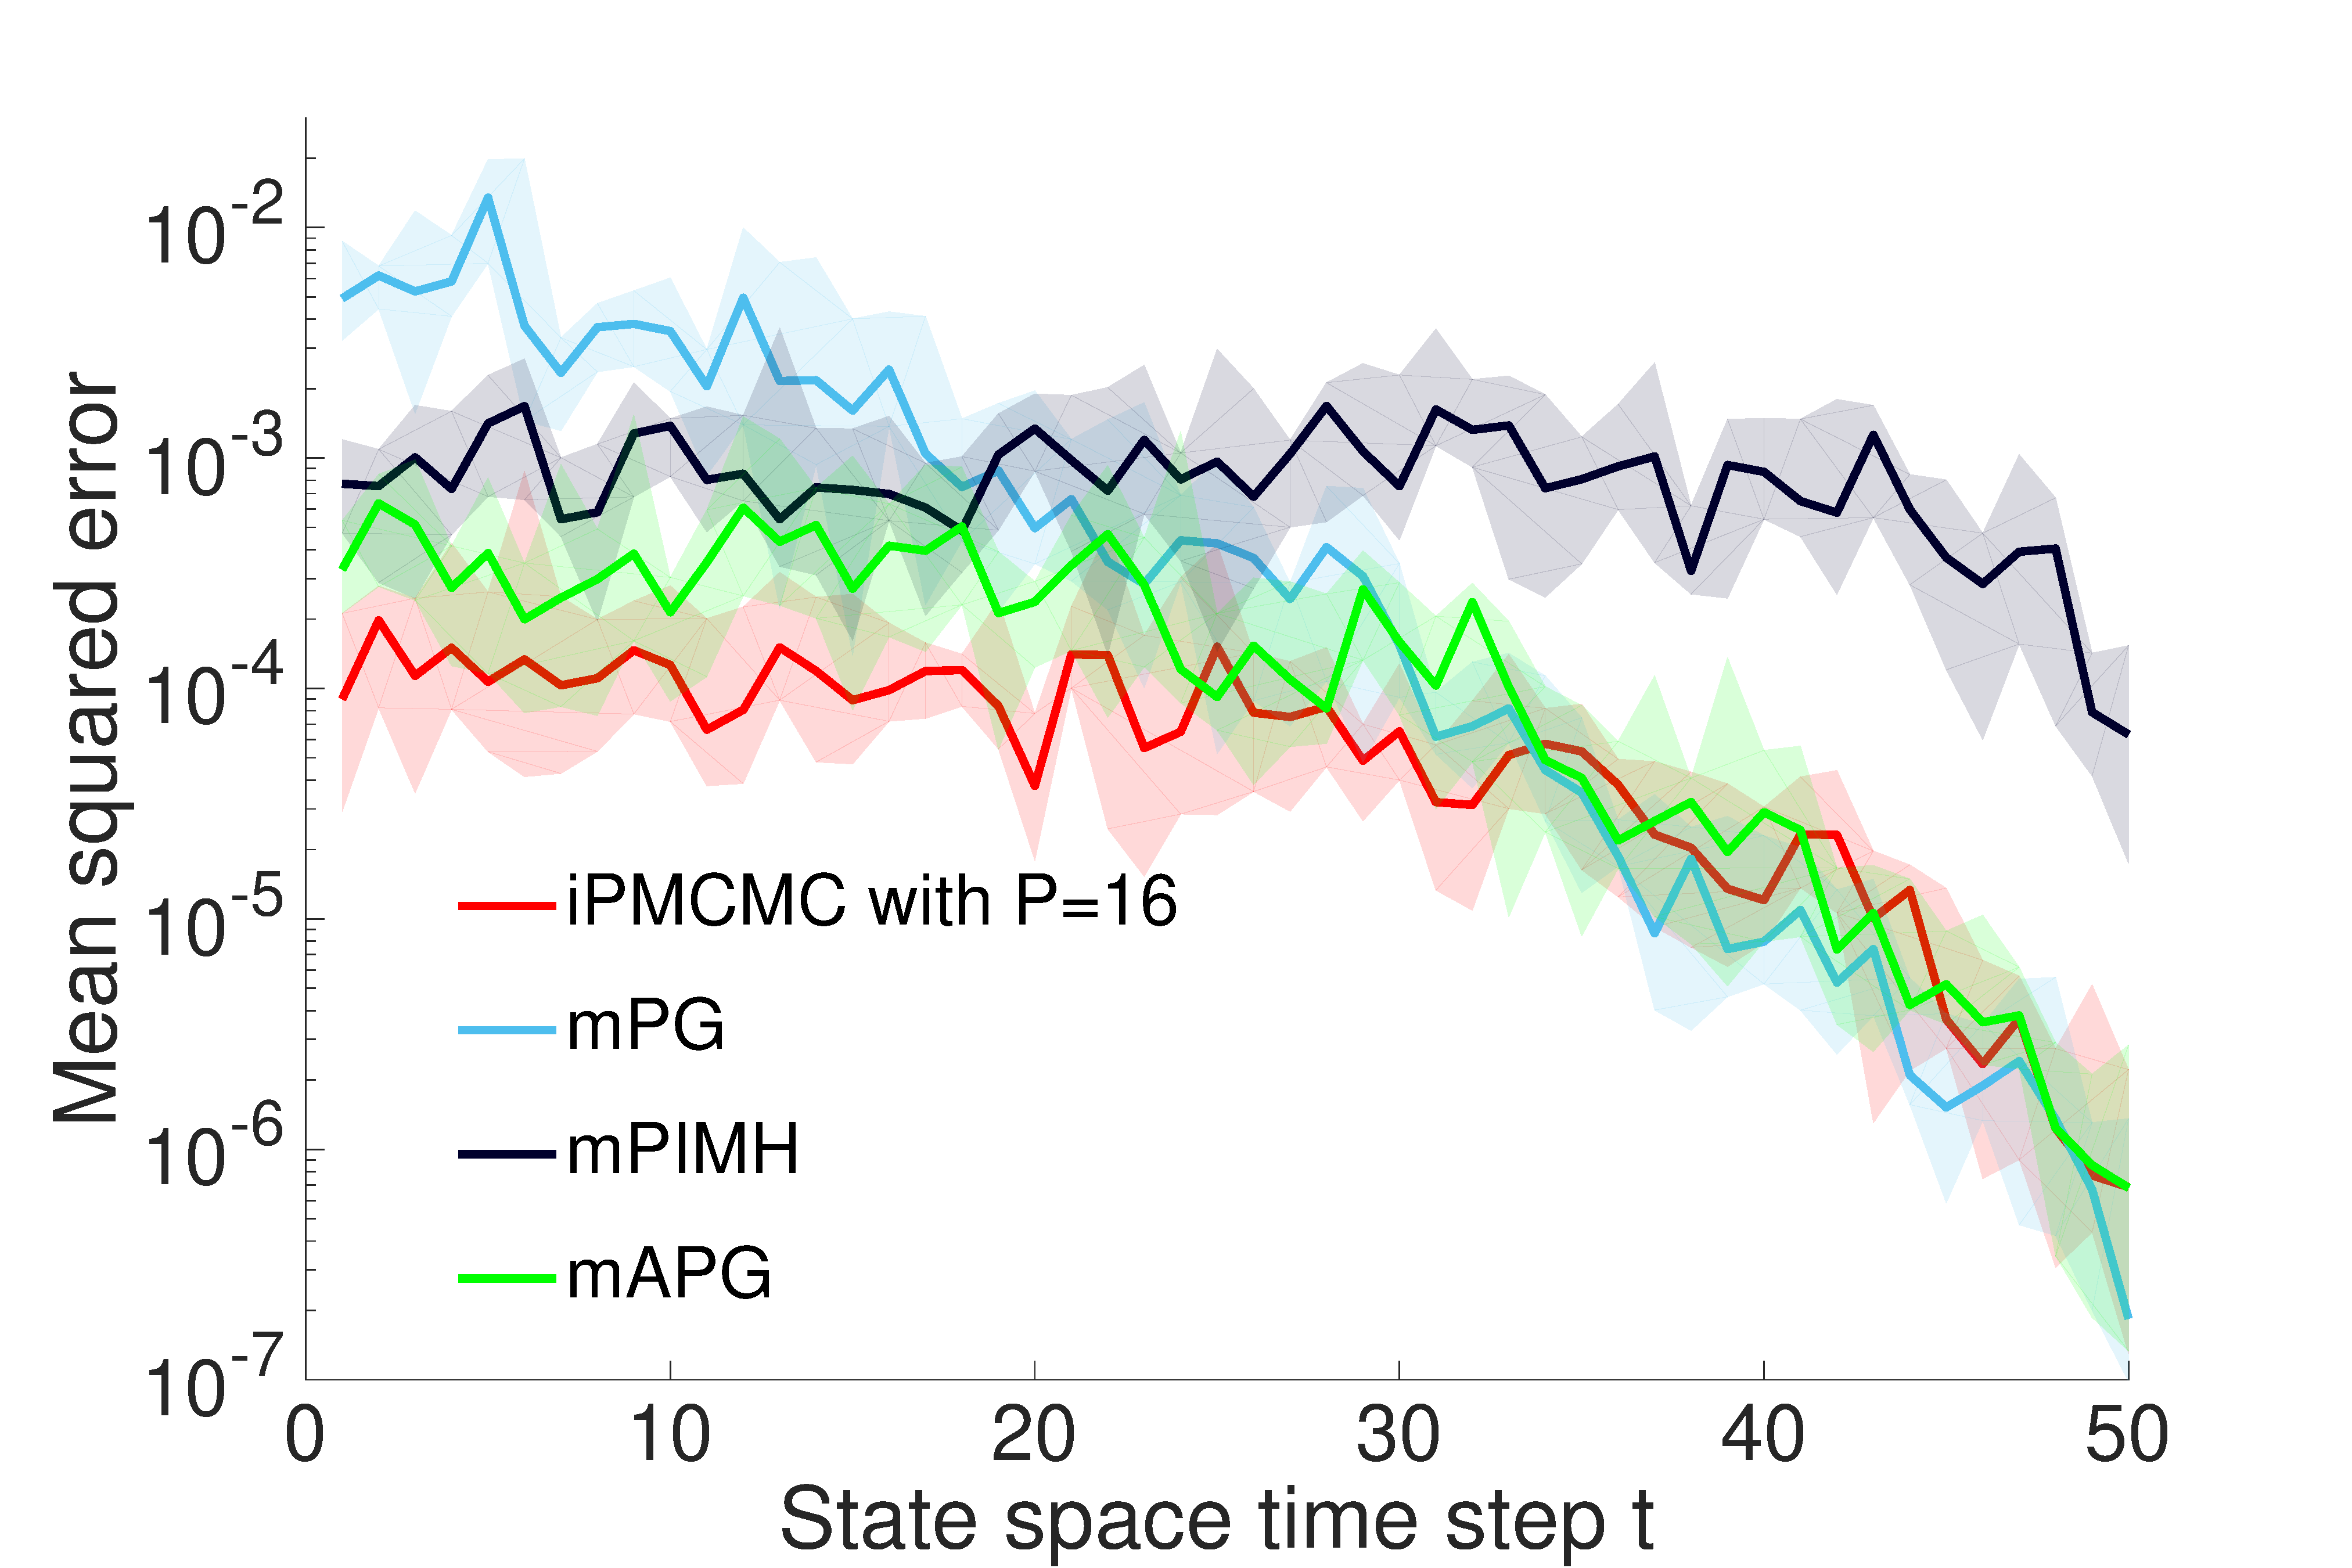
\includegraphics[width=0.98\textwidth]{mean_pos_lss}
		\caption{Final error in mean for latent marginals}
		\label{fig:meanPos}
	\end{subfigure}
	
	%	\begin{subfigure}[t]{0.49\textwidth}
	%		\includegraphics[width=\textwidth]{std_conv_lss}
	%		\caption{Convergence in standard deviation for full sequence}
	%		\label{fig:stdConv}
	%	\end{subfigure}
	%	~ %add desired spacing between images, e. g. ~, \quad, \qquad, \hfill etc. 
	%	%(or a blank line to force the subfigure onto a new line)
	%	\begin{subfigure}[t]{0.49\textwidth}
	%		\includegraphics[width=\textwidth]{std_pos_lss}
	%		\caption{Final error in standard deviation for latent marginals}
	%		\label{fig:stdPos}
	%	\end{subfigure}	
	\vspace{5pt}
	\caption{Mean squared error averaged over all dimensions and steps in the state sequence as a function of MCMC iterations (left) and mean squared error after $10^4$ iterations averaged over dimensions as function of position in the state sequence (right) for \eqref{eq:LGSS} with 50 time sequences.  The solid line shows the median error across the 10 tested synthetic datasets, while the shading shows the upper and lower quartiles.  Ground truth was calculated using the Rauch--Tung--Striebel smoother algorithm \cite{rauch1965maximum}. 
		\label{fig:groundTruth}}
\end{figure*}

Figure \ref{fig:meanConv} shows convergence (in MCMC iterations) in the estimate of the latent variable means to the ground-truth solution for iPMCMC and the benchmark algorithms.  It shows that iPMCMC comfortably outperforms the alternatives from around 200 iterations onwards, with only iPMCMC and mAPG demonstrating behaviour consistent with the Monte Carlo convergence rate, suggesting that mPG and mPIMH are still far from the ergodic regime.  Figure \ref{fig:meanPos} shows the same errors after $10^4$ MCMC iterations as a function of position in state sequence.  It demonstrates that iPMCMC outperformed all the other algorithms for the early stages of the state sequence, for which mPG performed particularly poorly. Toward the end of state sequence, iPMCMC, mPG and mAPG all gave similar performance, whilst that of mPIMH was significantly worse.

\begin{figure*}[t]
	\centering
	\begin{subfigure}[t]{0.49\textwidth}
		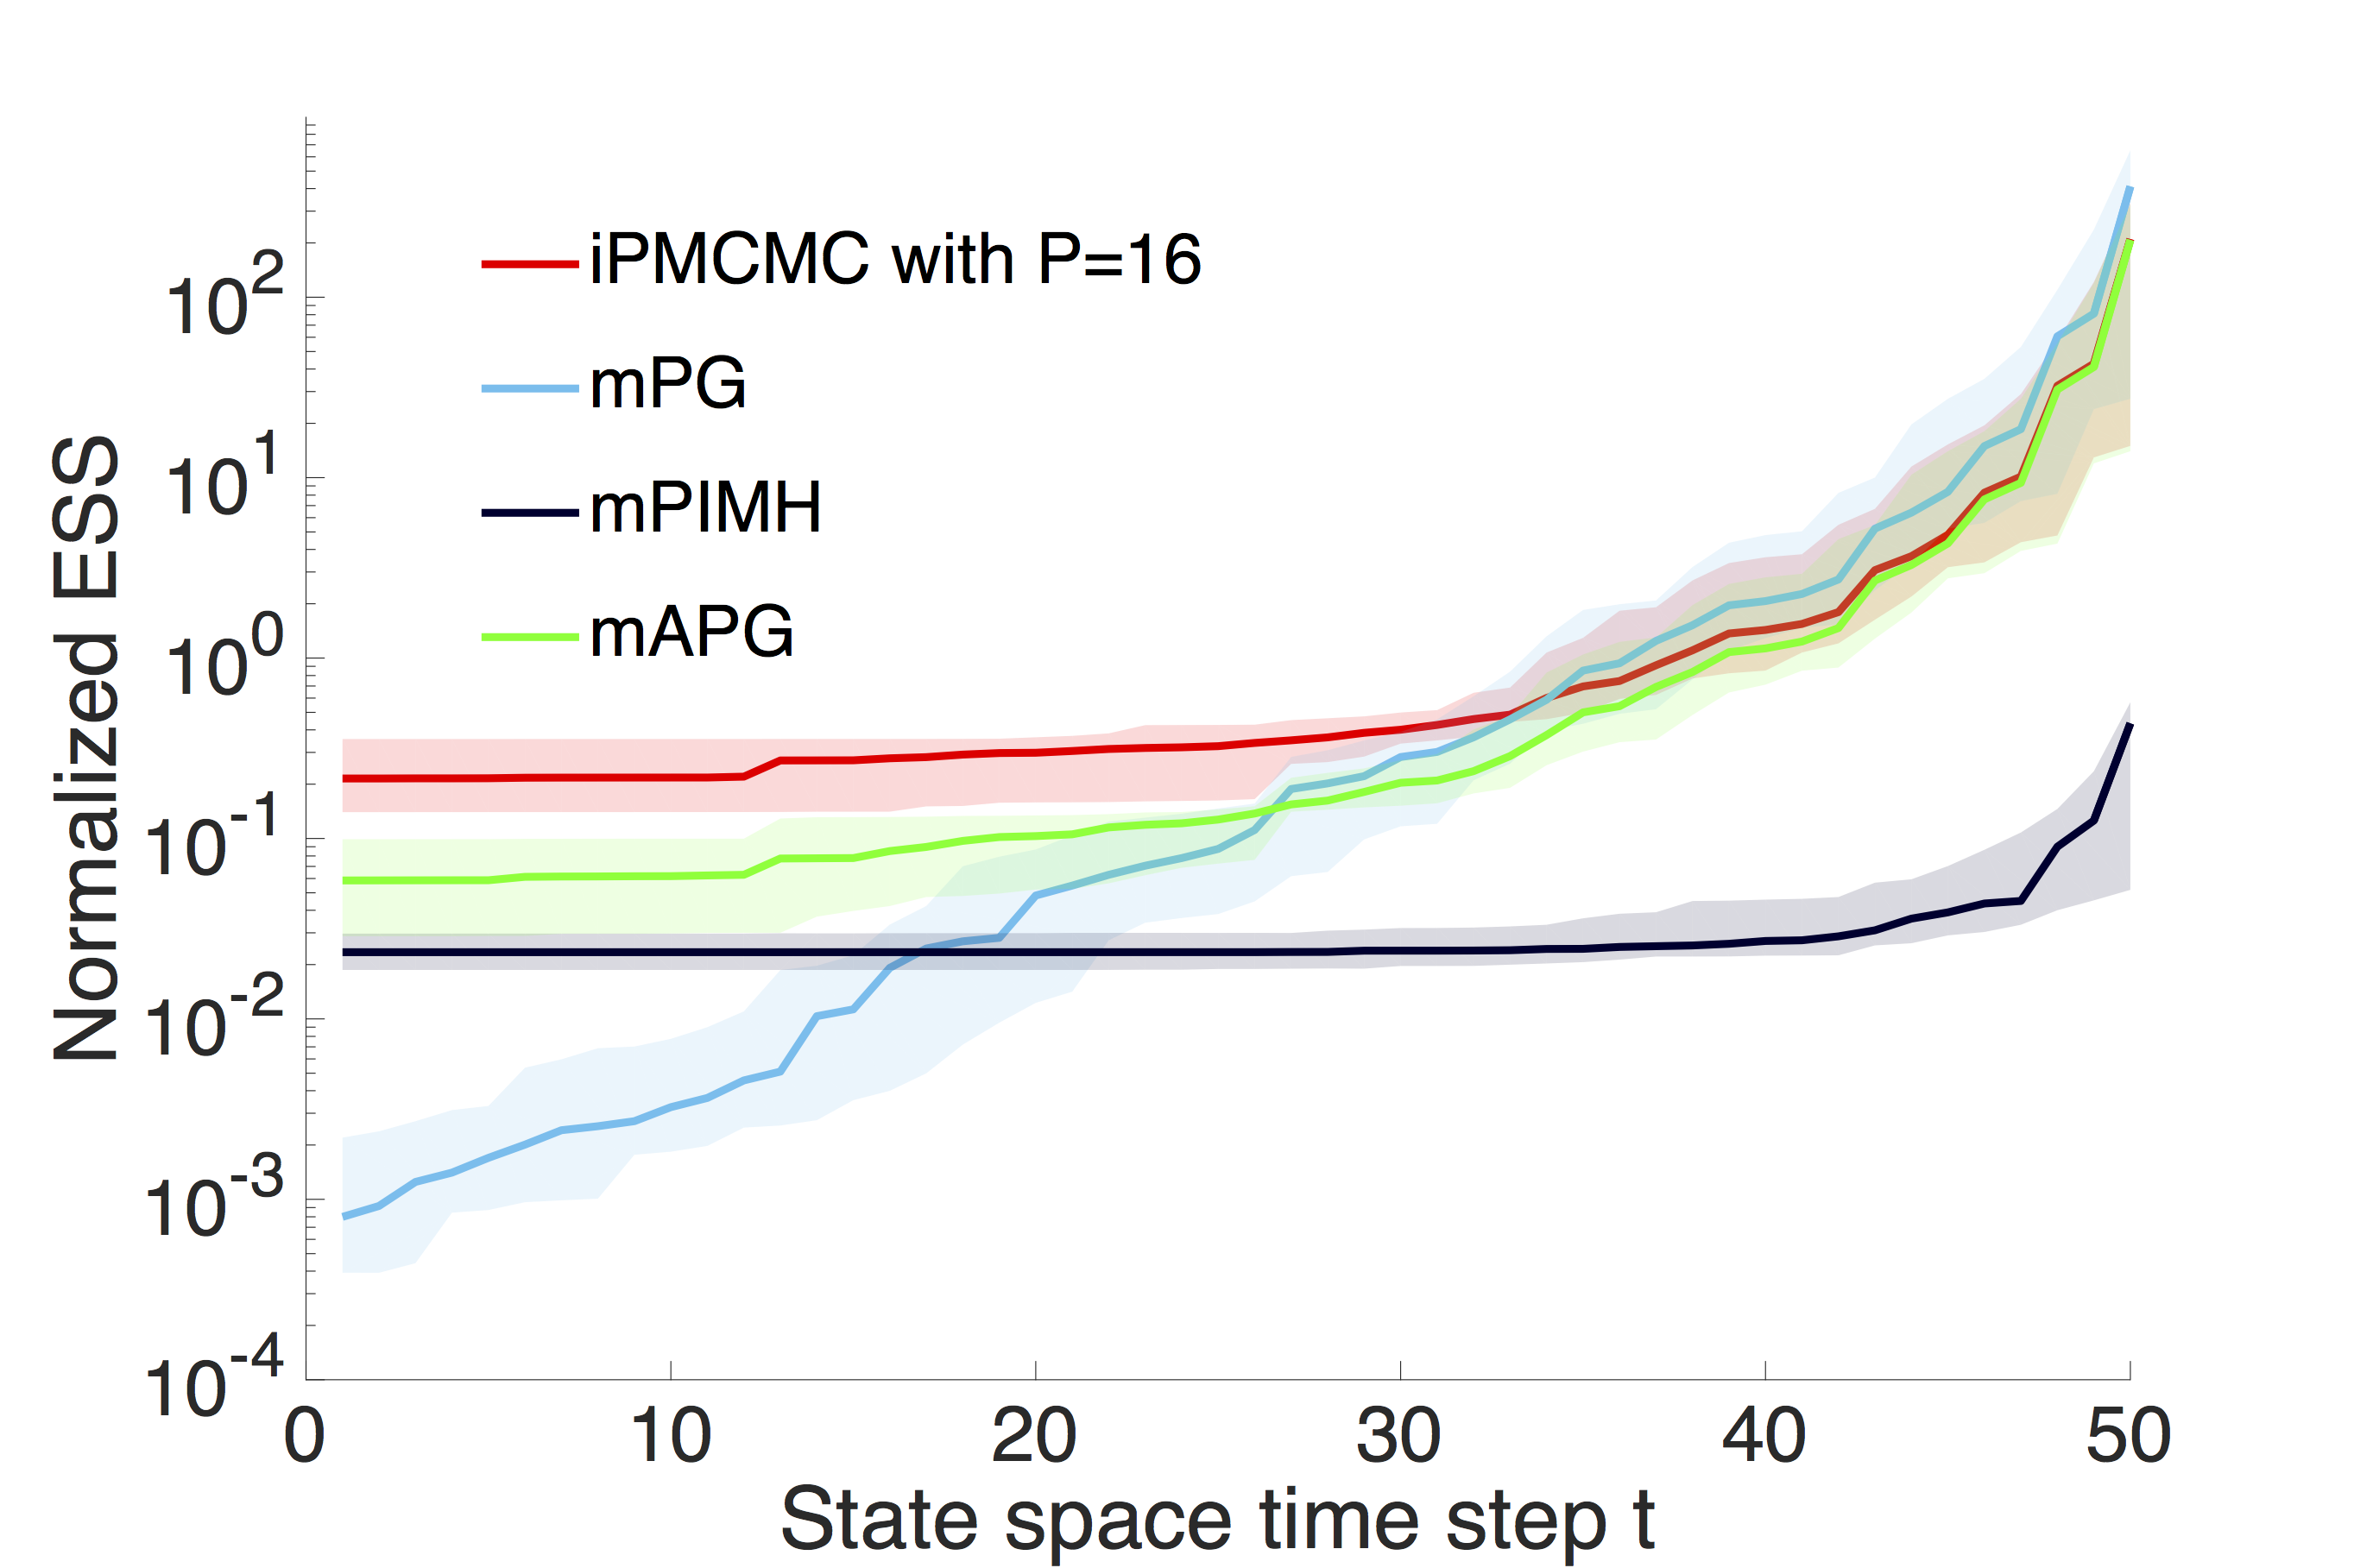
\includegraphics[width=\textwidth]{ess_lss}
		\caption{LGSSM}
	\end{subfigure}
	~ %add desired spacing between images, e. g. ~, \quad, \qquad, \hfill etc. 
	%(or a blank line to force the subfigure onto a new line)
	\begin{subfigure}[t]{0.49\textwidth}
		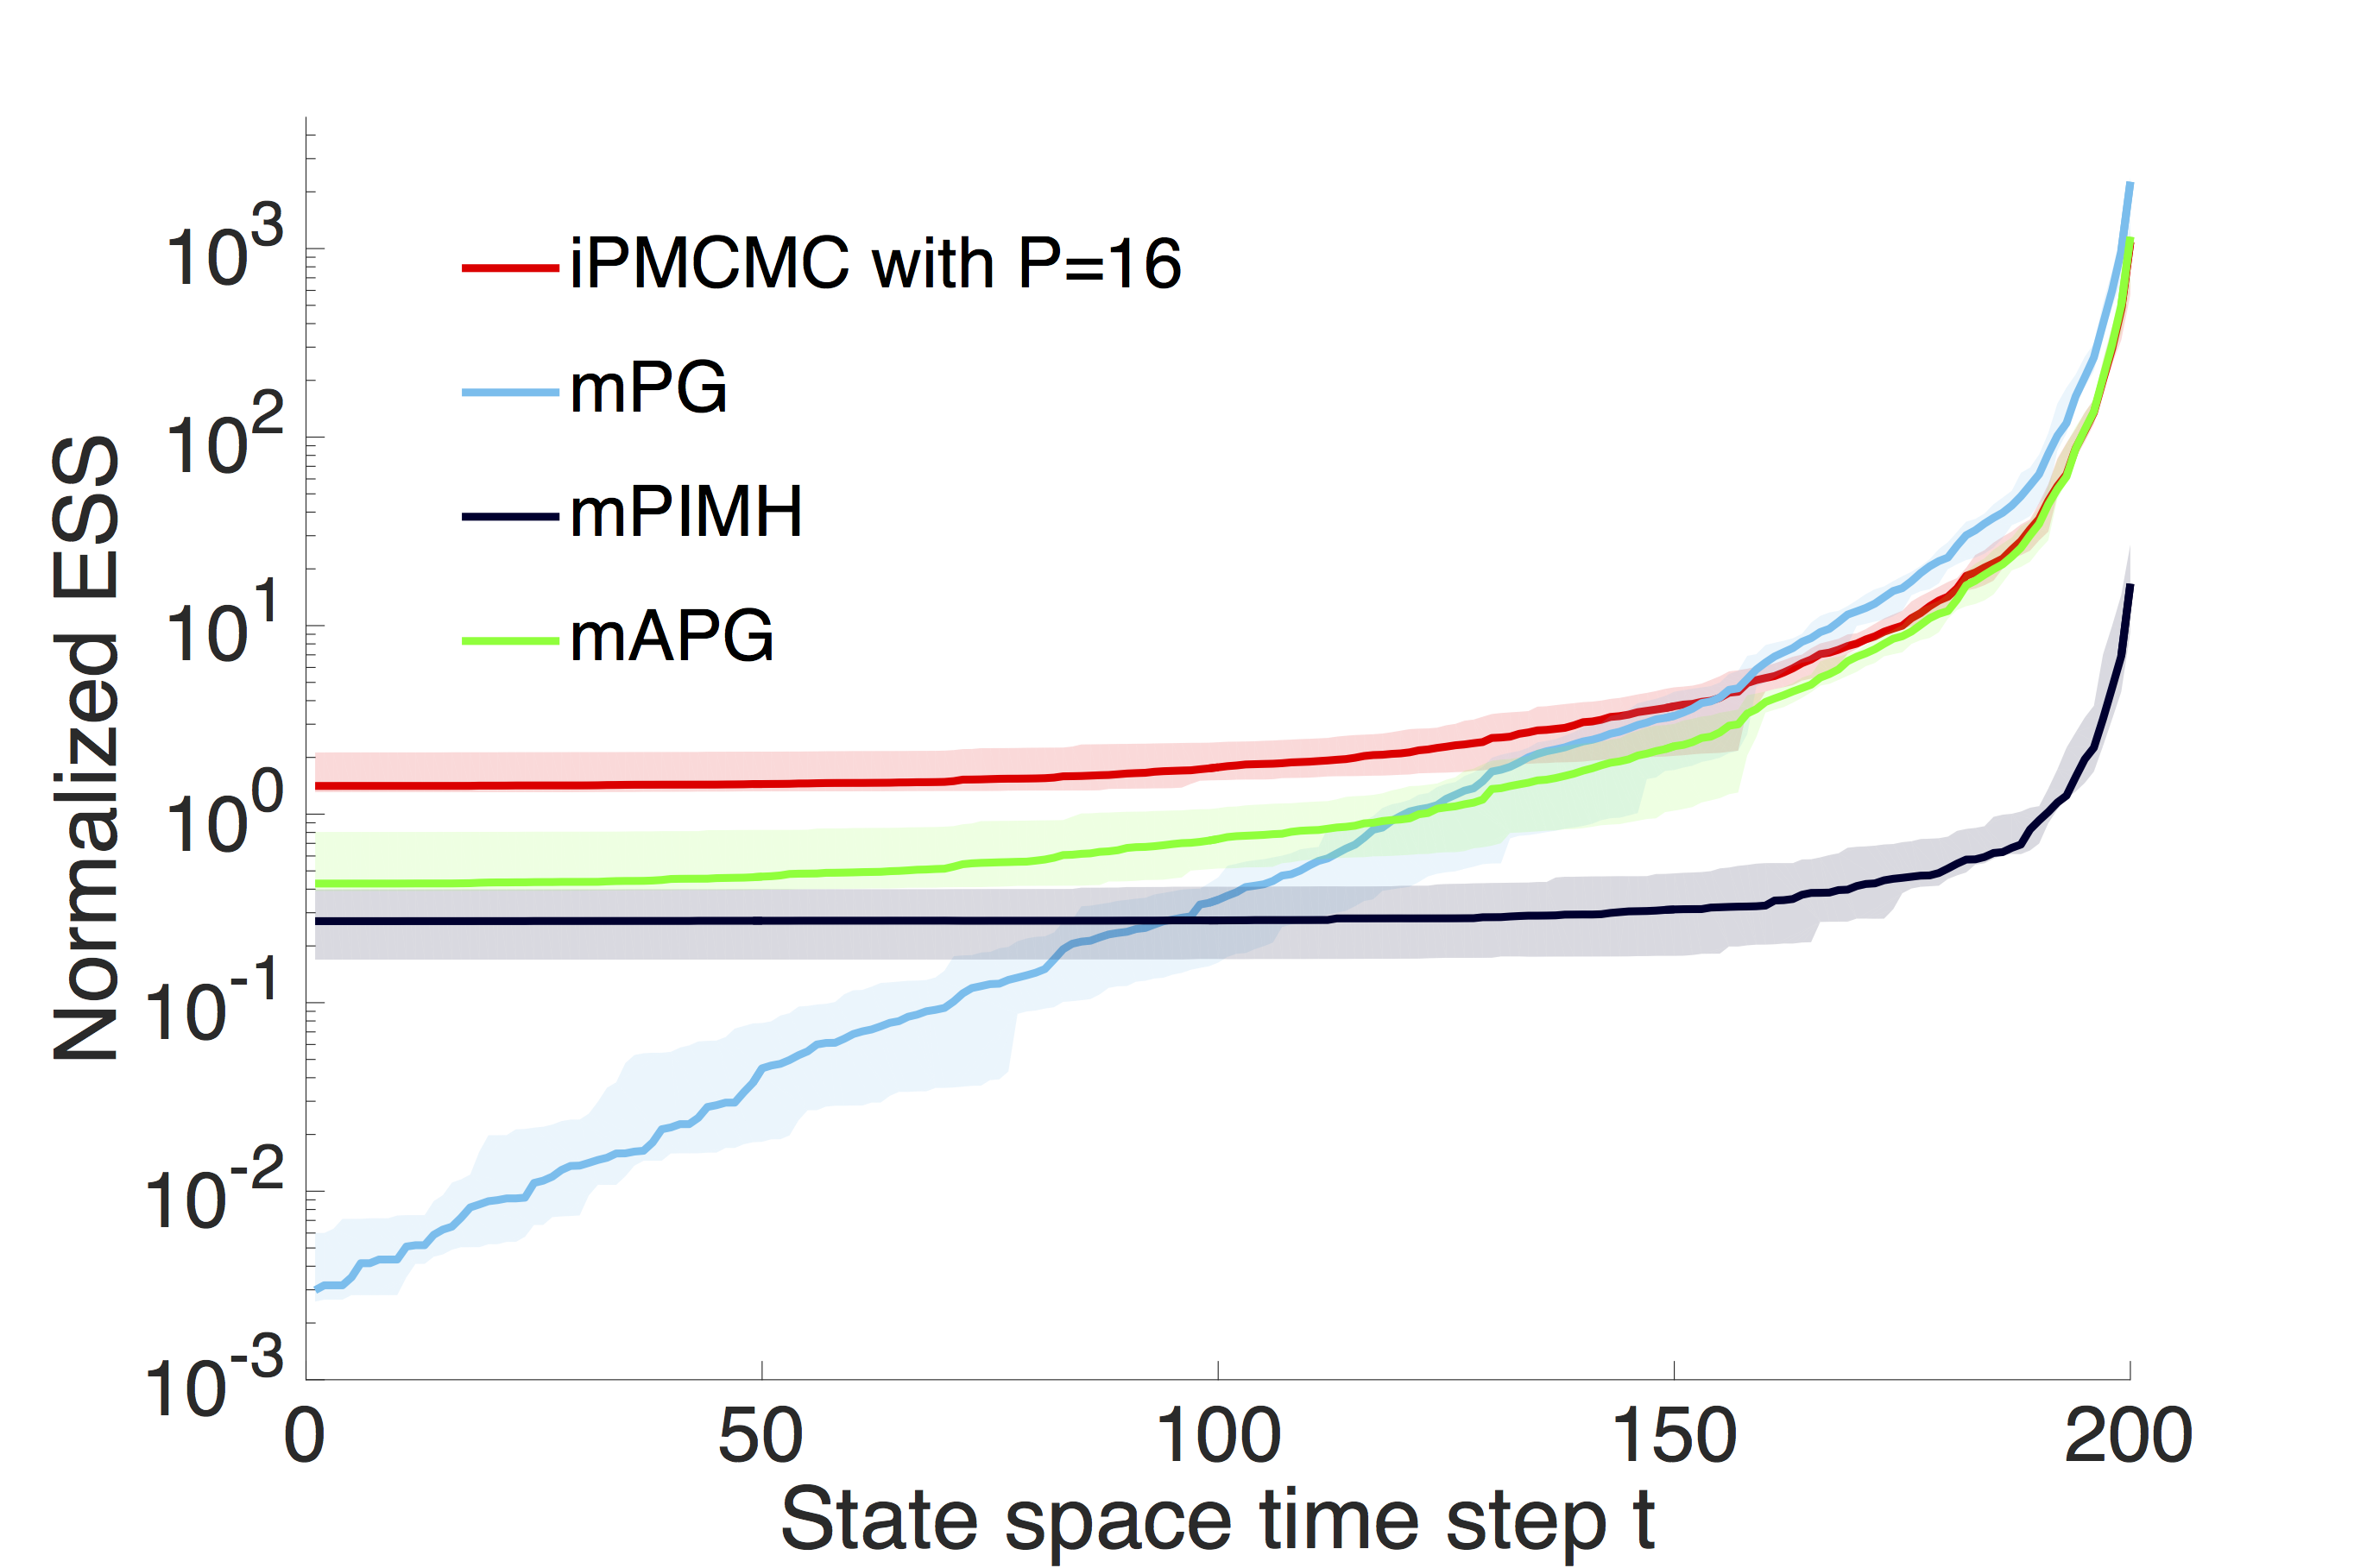
\includegraphics[width=\textwidth]{ess_nlss}
		\caption{NLSSM}
	\end{subfigure}
	\vspace{5pt}
	\caption{Normalized effective sample size  (NESS) for LGSSM (left) and NLSSM (right).
		\label{fig:ESS}}
	\vspace{-5pt}
\end{figure*}

\subsubsection{Nonlinear State Space Model}
\label{sec:nlss}

We next consider the one dimensional nonlinear state space model (NLSSM) considered by, among others, \citet{gordon1993novel,andrieuDH2010}
\begin{subequations}
	\label{eq:NLSS}
	\begin{align}
	x_1 & \sim \mathcal{N} \left(\mu, v^2\right) \label{eq:NLSSa} \displaybreak[0]\\
	x_t & = \frac{x_{t-1}}{2} + 25 \frac{x_{t-1}}{1+x_{t-1}^2} + 8 \cos \left(1.2t\right) + \delta_{t-1} \label{eq:NLSSb} \displaybreak[0]\\
	y_t & = \frac{{x_{t}}^2}{20} + \varepsilon_{t} \label{eq:NLSSc}
	\end{align}
\end{subequations}
where $\delta_{t-1} \sim \mathcal{N} \left(0, \omega^2\right)$ and $\varepsilon_{t} \sim \mathcal{N} \left(0, \sigma^2\right)$.  We set the parameters as $\mu = 0$, $v=\sqrt{5}$, $\omega = \sqrt{10}$ and $\sigma = \sqrt{10}$.  Unlike the LGSSM, this model does not have an analytic solution and therefore one must resort to approximate inference methods. 
% such as sampling.
Further, the multi-modal nature of the latent space makes full posterior inference over $x_{1:T}$ challenging for long state sequences. 

\begin{figure*}[t]
	\centering
	%\begin{subfigure}[t]{0.99\textwidth}
	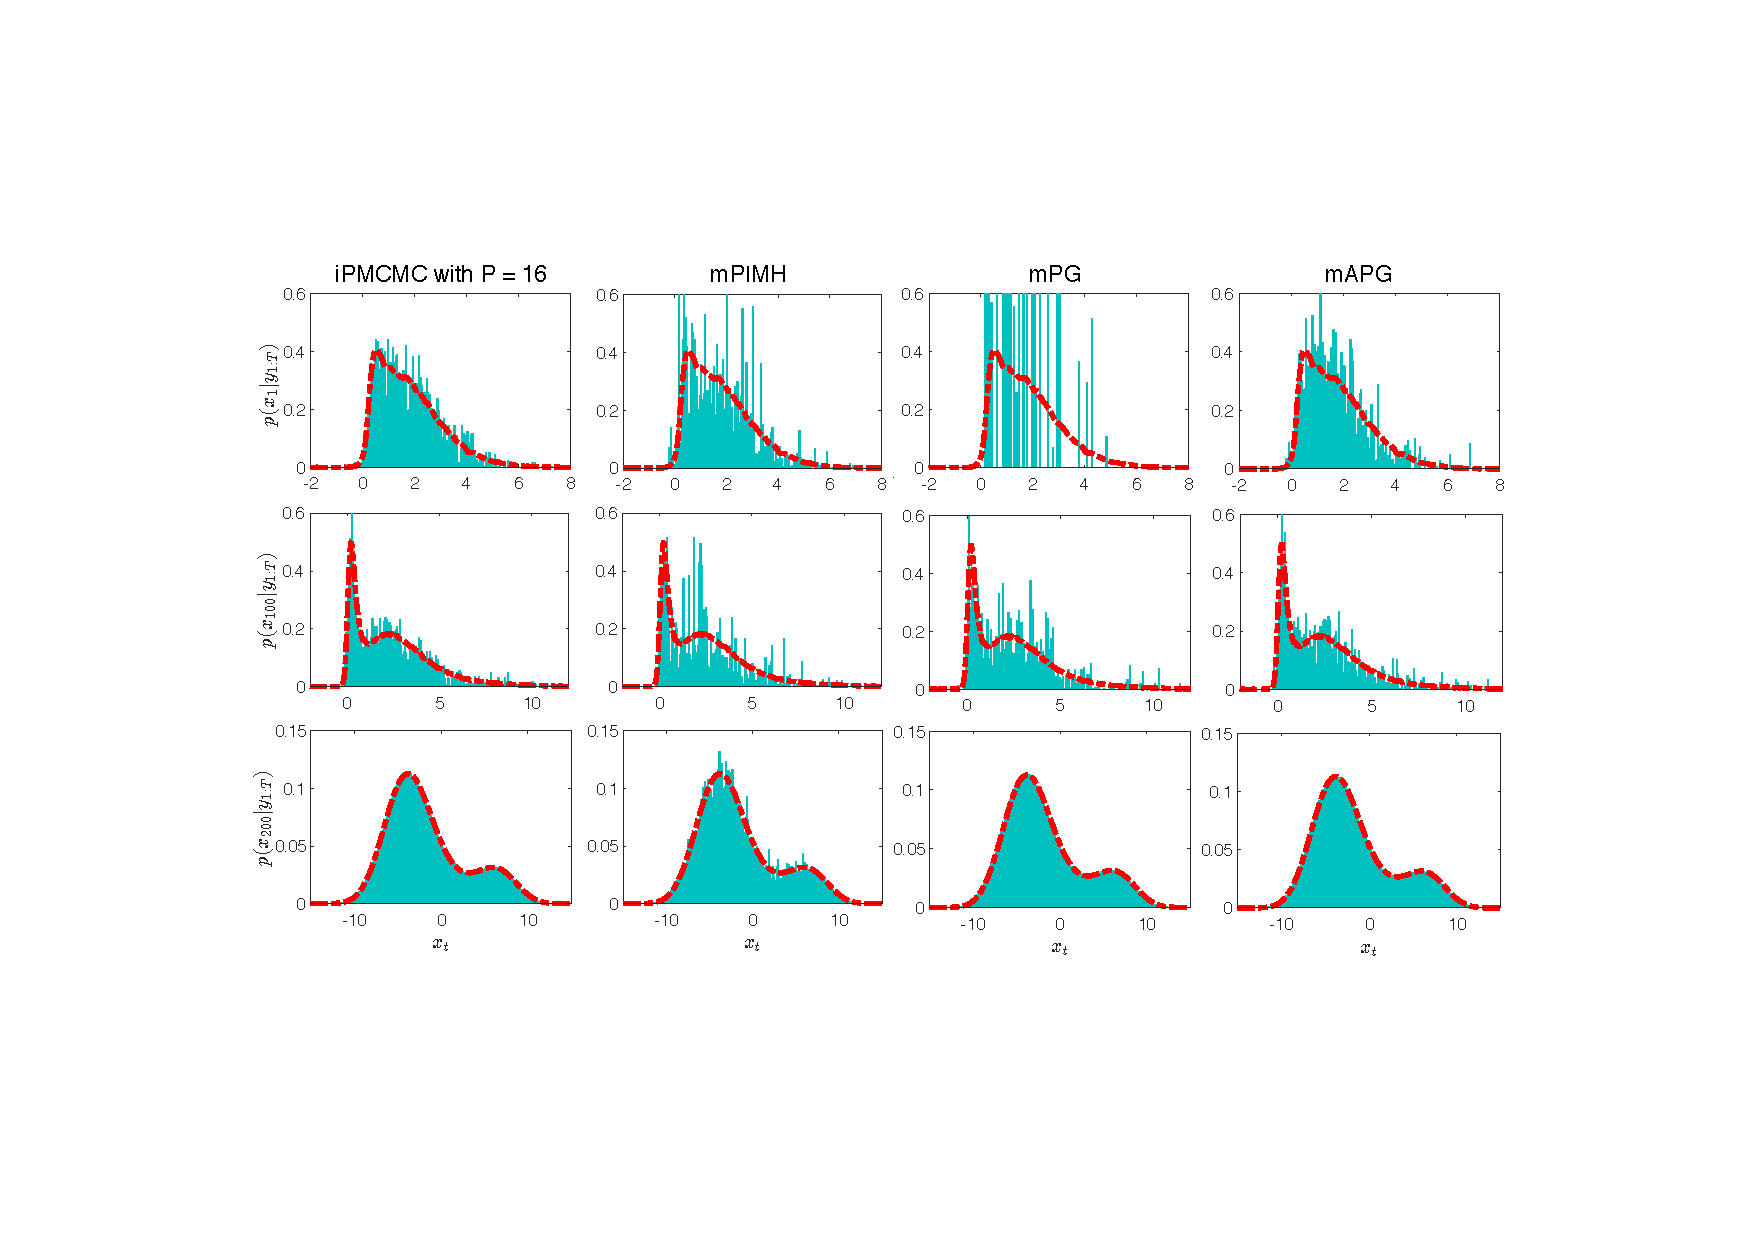
\includegraphics[width=1\textwidth]{nlss_histograms_minus_190.pdf}
	%\end{subfigure}
	\caption{Histograms of generated samples at $t=1, 100, \text{ and } 200$ for a single dataset generated from \eqref{eq:NLSS} with $T=200$.  Dashed red line shows an approximate estimate of the ground truth, found by running a kernel density estimator on the combined samples from a small number of independent SMC sweeps, each with $10^7$ particles. \label{fig:nlssHists}}
	\vspace{-10pt}
\end{figure*}

To examine the relative mixing of iPMCMC we calculate an effective sample size (ESS) for different steps in the state 
sequence as described in Section~\ref{sec:inf:foundation:ess}, taking care to  condensed identical samples.  To be
precise, let
\begin{align*}
u_{t}^k \in \{x_{t,m}^{i}[r]\}^{i=1:N,r=1:R}_{m=1:M}, \quad \forall k \in 1 \dots K, \; t \in 1 \dots T
\end{align*} 
denote the unique samples of $x_t$ generated by all the nodes and sweeps of particular algorithm after $R$ iterations, where $K$ is the total number of unique samples generated.  The weight assigned to these unique samples, $v_t^{k}$, is given by the combined weights of all particles for which $x_t$ takes the value $u_{t}^k$:
\begin{align}
v_t^{k} = \sum_{r=1}^{R} \sum_{m=1}^{M} \sum_{i=1}^{N} \bar{w}_{t,m}^{i,r} \eta_{m}^{r} \delta_{x_{t,m}^{i}[r]}(u_{t}^{k})
\end{align}
where $\delta_{x_{t,m}^{i}[r]}(u_{t}^{k})$ is the Kronecker delta function and $\eta_{m}^{r}$ is a node weight.  For iPMCMC the node weight is given by as per the Rao-Blackwellized estimator described in Section~\ref{sec:part:ipmcmc:allparticles}. For mPG and mPIMH, $\eta_{m}^{r}$ is simply $\frac{1}{RM}$,
as samples from the different nodes are weighted equally in the absence of interaction. 
Finally we define our effective sample size as $\text{ESS}_t = \left(\textstyle\sum_{k=1}^K \left(v_t^{k}\right)^2\right)^{-1}$.
%\begin{align}
%\label{eq:ESS}
%\text{ESS}_t = \left(\textstyle\sum_{k=1}^K \left(v_t^{k}\right)^2\right)^{-1}.
%\end{align}

Figure \ref{fig:ESS} shows the ESS for the LGSSM and NLSSM as a function of position in the state sequence.  For this, we omit the samples generated by the initialization step as this SMC sweep is common to all the tested algorithms.  We further normalize by the number of MCMC iterations so as to give an idea of the rate at which unique samples are generated.  These show that for both models the ESS of iPMCMC, mPG and mAPG is similar towards the end of the space sequence, but that iPMCMC outperforms all the other methods at the early stages. The ESS of mPG was particularly poor at early iterations.  PIMH performed poorly throughout, reflecting the very low observed acceptance ratio of around $7.3\%$ on average. 
%The lack of Monte Carlo convergence rate appearing in Figure \ref{fig:meanConv} also suggests this acceptance ratio is yet to converge, with the value in the ergodic regime likely to be even lower.   

It should be noted that the ESS is not a direct measure of performance for these models.  For example, the equal weighting of nodes is likely to make the ESS artificially high for mPG, mPIMH and mAPG, when compared with methods such as iPMCMC that assign a weighting to the nodes at each iteration.  To acknowledge this, we also plot histograms for the marginal distributions of a number of different position in the state sequence as shown in Figure \ref{fig:nlssHists}.  These confirm that iPMCMC and mPG have similar performance at the latter state sequence steps, whilst iPMCMC is superior at the earlier stages, with mPG producing almost no more new samples than those from the initialization sweep due to the degeneracy.  The performance of PIMH was consistently worse than iPMCMC throughout the state sequence, with even the final step exhibiting noticeable noise.

%An important feature of the ESS is that it is equal to the total number of samples ($NRM$) if all the samples are unique and have the same weight, and is equal to $1$ if there is only single unique sample with non-zero weight. It should be noted that ESS is not a direct measure of performance in the context of distributed PMCMC methods. In particular it takes no account of the suitability of the weights assigned to samples, for example the equal weighting assigned to different chains for mPG and mPIMH mean they will always have a higher ESS for a particle sweep \brooks{clarify ``particle sweep''?} than a iPMCMC sweep generating the same samples, regardless of whether this equal weighting gives a better approximation to the true posterior. \fredrik{I did not quite understand the last sentence.}
